\documentclass[a4paper,12pt]{report}

\usepackage{cmap}
\usepackage[T2A]{fontenc}
\usepackage[utf8]{inputenc}
\usepackage[english,russian]{babel}
\usepackage{listings}
\usepackage{amsmath}
\usepackage{amsfonts}
\usepackage{float}
\usepackage{csquotes}
\usepackage{hyphenat}

% \usepackage{titlesec}
% \newcommand{\sectionbreak}{\clearpage}

\usepackage{graphicx}
\graphicspath{ {./images/} }

\usepackage{xcolor}
% \usepackage{courier}

\usepackage[
    backend=biber,
    style=alphabetic,
    sorting=ynt
]{biblatex}
\addbibresource{resources.bib}

\definecolor{buzzlightyear}{HTML}{8757A5}
\definecolor{grass}{HTML}{738D06}
\definecolor{sand}{HTML}{F18A2B}
\definecolor{comment}{HTML}{8E908B}

\lstdefinestyle{habrstyle}{
    backgroundcolor=\color{white},   
    commentstyle=\color{comment},
    keywordstyle=\bfseries\color{buzzlightyear},
    numberstyle=\tiny\color{comment},
    stringstyle=\color{grass},
    basicstyle=\ttfamily\footnotesize,
    breakatwhitespace=false,         
    breaklines=true,                 
    captionpos=b,                    
    keepspaces=true,                 
    numbers=left,                    
    numbersep=5pt,                  
    showspaces=false,                
    showstringspaces=false,
    showtabs=false,                  
    tabsize=4
}

\lstset{style=habrstyle}

\author{Луняк Николай}
\title{Лабораторная работа 4}
\date{\today}

\begin{document}
    \maketitle
    \tableofcontents
    \listoffigures
    \lstlistoflistings
    
    \chapter{Свойства преобразования Фурье}
    
    \section{Общее}
    
    На последней лекции Наталья Владимировна попросила добавить в ближайший отчет описание свойств преобразования Фурье, что и будет сделано в данном разделе.
    
    О том, что такое само по себе преобразование Фурье, мы говорили на лекции, однако в качестве еще одного источника возможной интуиции мне показался примечательным ролик \sloppy{\texttt{3Blue1Brown}} \cite{furv}.
    
    Пусть формулы тоже будут под рукой. Для сигнала $f(t)$:

    % \begin{align}
    %     \text{прямое: } && F(\nu) &= \int_{-\infty}^{\infty} f(t) e^{-2\pi i\nu t} dt \\
    %     \text{обратное: } && f(t) &=  \int_{-\infty}^{\infty} F(\nu) e^{2\pi i\nu t} d\nu
    % \end{align}
    
    \[
        \begin{aligned}
            \text{Прямое: } && F(\nu) &= \int_{-\infty}^{\infty} f(t) e^{-2\pi i\nu t} dt \\
            \text{Обратное: } && f(t) &=  \int_{-\infty}^{\infty} F(\nu) e^{2\pi i\nu t} d\nu
        \end{aligned}
    \]
    
    \section{Свойства}
    
    \subsection{Линейность}
    
    По определению, для некоторого векторного пространства $(V,K,+,\cdot)$, $a,b \in V$, $\gamma \in K$:
    
    \[
        \begin{aligned}
            f: V \rightarrow V \text{ - линейна}
            \Longleftrightarrow
            \begin{cases}
                    \gamma\cdot f(a) = f(\gamma\cdot a) \\
                    f(a) + f(b) = f(a + b)
            \end{cases}
        \end{aligned}
    \]
    
    Очевидно, ПФ удовлетворяет этому условию (как функция на $(\mathbb{R} \rightarrow \mathbb{R},\mathbb{C},+,\cdot)$), а следовательно:
    
    \[
        \begin{aligned}
            Fourier\left(\sum_{i}\alpha_i\phi_i(t)\right)
            &= \sum_{i}\alpha_i \cdot Fourier(\phi_i(t)) \\
            &= \sum_{i}\alpha_i \Phi_i(\nu)
        \end{aligned}
    \]
    
    \subsection{Смещение функции}
    
    При смещении нашей подопытной функции $\phi(t)$ на $\Delta t$ результат ПФ умножается на $e^{2\pi i \nu\Delta t}$. Пусть $t' = t + \Delta t$, тогда:
    
    \[
        \begin{aligned}
            Fourier\left(\phi(t + \Delta t)\right)
            &= \int_{-\infty}^{\infty} \phi(t + \Delta t) e^{-2\pi i\nu t} dt \\
            &= \int_{-\infty}^{\infty} \phi(t') e^{-2\pi i\nu (t' - \Delta t)} dt
        \end{aligned}
    \]
    
    Так как $dt' = d(t + \Delta t) = dt$, то:
    
    \[
        \begin{aligned}
            \int_{-\infty}^{\infty} \phi(t') e^{-2\pi i\nu (t' - \Delta t)} dt'
            &= e^{2\pi i\nu\Delta t} \cdot \int_{-\infty}^{\infty} \phi(t') e^{-2\pi i\nu t'} dt' \\
            &= e^{2\pi i\nu\Delta t} \cdot F(\nu)
        \end{aligned}
    \]
    
    \subsection{Масштабирование функции}
    
    Аналогично, $t' = \alpha t$:
    
    \[
        \begin{aligned}
            Fourier\left(\phi(\alpha t)\right)
            &= \int_{-\infty}^{\infty} \phi(\alpha t) e^{-2\pi i\nu t} dt \\
            &= \int_{-\infty}^{\infty} \phi(t') e^{-2\pi i\nu \frac{t'}{\alpha}} dt
        \end{aligned}
    \]
    
    Так как $dt' = \alpha dt$, то для $a > 0$:
    
    \[
        \begin{aligned}
            \int_{-\infty}^{\infty} \phi(t') e^{-2\pi i\nu \frac{t'}{\alpha}} dt
            &= \frac{1}{\alpha} \int_{-\infty}^{\infty} \phi(t') e^{-2\pi i\frac{\nu}{\alpha} t'} dt \\
            &= \frac{1}{\alpha} \Phi\left(\frac{\nu}{\alpha}\right)
        \end{aligned}
    \]
    
    А вот для $a < 0$ мы получим $dt' < 0$ при $dt > 0$. Тогда надо поменять местами пределы интегрирования и выскочит минус в результате:
    
    \[
        \begin{aligned}
            -\frac{1}{\alpha} \Phi\left(\frac{\nu}{\alpha}\right)
        \end{aligned}
    \]
    
    Тогда в одной форме это:
    
    \[
        \begin{aligned}
            \frac{1}{\left|\alpha\right|} \Phi\left(\frac{\nu}{\alpha}\right)
        \end{aligned}
    \]
    
    Вывод: при сжатии функции по времени в $\alpha$ раз, ее ПФ расширяется по частоте в $\alpha$ раз.
    
    \subsection{Перемножение функции}
    
    ПФ произведения двух функций - это свертка их ПФ.
    
    \[
        \begin{aligned}
            Fourier\left(\phi(t)\xi(t)\right) 
            &= \int_{-\infty}^{\infty} \phi(t)\xi(t) e^{-2\pi i\nu t} dt \\
            &= \int_{-\infty}^{\infty} \left( \int_{-\infty}^{\infty} \Phi(k) e^{2\pi i kt} dk \right) \xi(t) e^{-2\pi i\nu t} dt \\
            &= \int_{-\infty}^{\infty} \Phi(k) \left( \int_{-\infty}^{\infty} \xi(t) e^{2\pi i (k - \nu)t} dt \right) dk \\
            &= \int_{-\infty}^{\infty} \Phi(k) \left( \int_{-\infty}^{\infty} \xi(t) e^{-2\pi i (\nu - k)t} dt \right) dk \\
            &= \int_{-\infty}^{\infty} \Phi(k) \Xi(\nu - k) dk \\
            &= \left(\Phi * \Xi\right)(\nu)
        \end{aligned}
    \]
    
    \subsection{Свертывание функции}
    
    ПФ свертки двух функций есть произведение ПФ этих функций. Доказывается аналогично в силу \textquote{симметрии} прямого и обратного преобразований Фурье.
    
    \subsection{Дифференциирование функции}
    
    При дифференциировании $\phi(t)$ по $t$ ее ПФ умножается на $2\pi i \nu$.
    
    \[
        \begin{aligned}
            Fourier\left(\frac{d\phi(t)}{dt}\right) 
            &= \int_{-\infty}^{\infty} \frac{d\phi(t)}{dt} e^{-2\pi i\nu t} dt \\
            &= \int_{-\infty}^{\infty} e^{-2\pi i\nu t} d\phi(t) \\
            &= \phi(t) e^{-2\pi\nu t} \bigg|_{-\infty}^{\infty} - \int_{-\infty}^{\infty} \phi(t) d\left(e^{-2\pi i\nu t}\right) \\
            &= \phi(t) e^{-2\pi\nu t} \bigg|_{-\infty}^{\infty} + 2\pi i\nu \int_{-\infty}^{\infty} \phi(t) e^{-2\pi i\nu t} dt \\
            &= \phi(t) e^{-2\pi\nu t} \bigg|_{-\infty}^{\infty} + 2\pi i\nu \cdot \Phi(\nu) \\
        \end{aligned}
    \]
    
    Прямое и обратное преобразование Фурье существует для функций с органиченной энергией, то есть:
    
    \[
        \begin{aligned}
            \int_{-\infty}^{\infty} |\phi(t)|^2 dt \neq \infty
        \end{aligned}
    \]
    
    И из этого следует, что первое слагаемое должно быть 0.
    
    \subsection{Интегрирование функции}
    
    Как можно предположить, тут произойдет обратное - деление на эту величину. Правда, теперь мы еще требуем, чтобы в функции не было константной составляющей (при дифференциировании она бы пропала, а вот при интегрировании - нет).
    
    \[
        \begin{aligned}
            Fourier\left(\int_{-\infty}^{t} \phi(t') dt'\right) 
            &= \int_{-\infty}^{\infty} \left( \int_{-\infty}^{t} \phi(t') dt' \right) e^{-2\pi i\nu t} dt \\
            &= -\frac{1}{2\pi i\nu} \cdot \int_{-\infty}^{\infty} \left( \int_{-\infty}^{t} \phi(t') dt' \right) d\left(e^{-2\pi i\nu t}\right) \\
            &= -\frac{1}{2\pi i\nu} \cdot \left[ e^{-2\pi i\nu t} \int_{-\infty}^{t} \phi(t') dt' \biggr|_{-\infty}^{\infty} - \int_{-\infty}^{\infty} e^{-2\pi i\nu t} d\left(\int_{-\infty}^{t} \phi(t') dt'\right)\right] \\
            &= -\frac{1}{2\pi i\nu} \cdot \left[ e^{-2\pi i\nu t} \int_{-\infty}^{t} \phi(t) dt \biggr|_{-\infty}^{\infty} - \int_{-\infty}^{\infty} e^{-2\pi i\nu t} \phi(t) dt\right] \\
            &= -\frac{1}{2\pi i\nu} \cdot \left[ 0 - \int_{-\infty}^{\infty} e^{-2\pi i\nu t} \phi(t) dt\right] \\
            &= \frac{1}{2\pi i\nu} \cdot \int_{-\infty}^{\infty} e^{-2\pi i\nu t} \phi(t) dt \\
            &= \frac{1}{2\pi i\nu} \cdot \Phi(\nu)
        \end{aligned}
    \]
    
    А 0 там появился из-за того, что $\int_{-\infty}^{\infty} \phi(t') dt' = 0$.
    
    \subsection{Обратимость}
    
    Ну и само собой то, что прямой и обратное преобразование Фурье - два брата-близнеца с точностью до знака.
    
    \chapter{Пробуем примеры из \textquote{A Soft Murmur}}
    
    Скачиваем с сайта три файла и смотрим на их спектры.
    
\begin{lstlisting}[language=Python,caption=Анализ файлов]
from thinkdsp import Signal, Sinusoid, SquareSignal, TriangleSignal, SawtoothSignal, ParabolicSignal
from thinkdsp import normalize, unbias, PI2, decorate
from thinkdsp import Chirp
from thinkdsp import read_wave

import numpy as np

from matplotlib import pyplot

files = [
    'Sounds/169289__qubodup__gong-bell-monkay-s-singing-bowl-modified.wav',
    'Sounds/22604__martypinso__dmp010037-crickets-texas.wav',
    'Sounds/136977__audionautics__crowd-long.wav',
]

def analyze(file):
    print(f'Analyzing "{file}"')
    wave = read_wave(file)
    segment = wave.segment(start=0, duration=5)
    pyplot.title('Waveform')
    segment.plot()
    pyplot.show()

    spectrum = segment.make_spectrum()
    
    pyplot.title('Spectrum (Linear Scale)')
    spectrum.plot_power()
    decorate(
        xlabel='Frequency (Hz)',
        ylabel='Power',
    )
    pyplot.show()
    
    pyplot.title('Spectrum (Log-Log Scale)')
    spectrum.plot_power(linewidth=0.5)
    loglog = dict(xscale='log', yscale='log')
    decorate(
        xlabel='Frequency (Hz)',
        ylabel='Power',
        **loglog
    )
    pyplot.show()
    
    pyplot.title('Spectrogram')
    segment.make_spectrogram(512).plot(high=5000)
    pyplot.show()
    
    return segment.make_audio()

[analyze(it) for it in files]
\end{lstlisting}

    В изображениях ниже присутствует опечатка: те, что подписаны как \textquote{Amplitude}, являются так же квадратом амплитуды, просто они отражены не в \textquote{log-log scale}, а те, что подписаны как \textquote{Power}, являются квадратом амплитуды, отраженном как раз в логарифмическом масштабе. Ввиду некомфортности работы с изображниями в \LaTeX, я решил их не исправлять.

    Начнем с гонга.

    \begin{figure}[H]
        \centering
        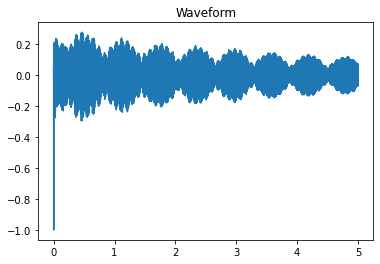
\includegraphics[width=0.75\textwidth]{ex1_gong_wave.png}
        \caption{Гонг}
        \label{fig:ex1_gong_wave}
    \end{figure}
    
    \begin{figure}[H]
        \centering
        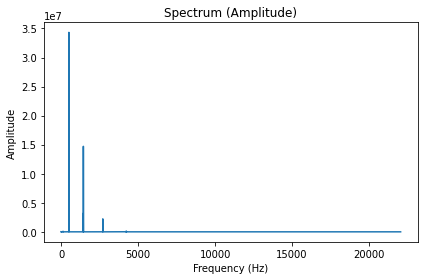
\includegraphics[width=0.75\textwidth]{ex1_gong_spectrum_amplitude.png}
        \caption{Спектр гонга (линейный масштаб)}
        \label{fig:ex1_gong_spectrum_amplitude}
    \end{figure}
    
    Большие значения аплитуды соответствуют малым значениям частоты, что дает основания полагать, что это \textquote{красный} bkb \textquote{розовый} шум, хотя наличие всего лишь трех \textquote{пиков} можно с натяжкой считать настоящим шумом, но такой уж файл скачался...
    
    \begin{figure}[H]
        \centering
        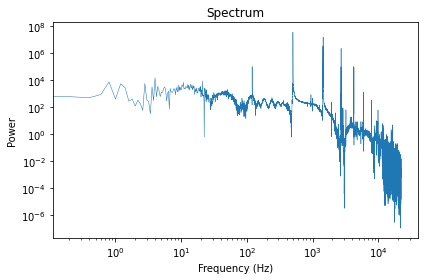
\includegraphics[width=0.75\textwidth]{ex1_gong_spectrum.png}
        \caption{Спектр гонга (логарифмический масштаб)}
        \label{fig:ex1_gong_spectrum}
    \end{figure}
    
    \begin{figure}[H]
        \centering
        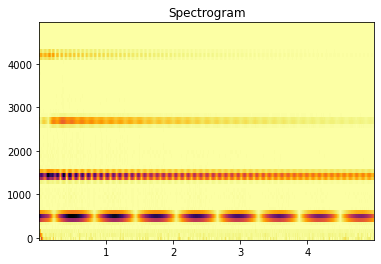
\includegraphics[width=0.75\textwidth]{ex1_gong_spectrogram.png}
        \caption{Спектрограмма гонга}
        \label{fig:ex1_gong_spectrogram}
    \end{figure}
    
    В спектрограмме виднеется определенный периодический \textquote{шаблон}, а также присутствуют лишь определенные частоты, которые мы видели ранее, что четко дает понять, что мы работаем не с шумом, а со сигналом, обладающим стабильным четким \textquote{временным профилем}.
    
    \begin{figure}[H]
        \centering
        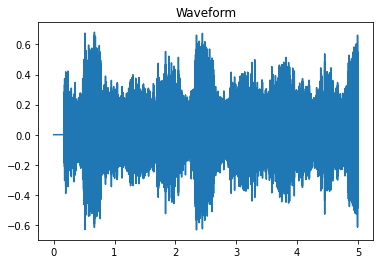
\includegraphics[width=0.75\textwidth]{ex1_crickets_wave.png}
        \caption{Сверчки}
        \label{fig:ex1_crickets_wave}
    \end{figure}
    
    \begin{figure}[H]
        \centering
        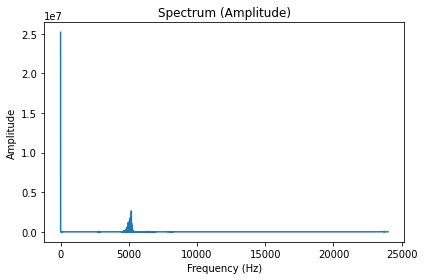
\includegraphics[width=0.75\textwidth]{ex1_crickets_spectrum_amplitude.png}
        \caption{Спектр сверчков (линейный масштаб)}
        \label{fig:ex1_crickets_spectrum_amplitude}
    \end{figure}
    
    Приблизим этот фрагмент, отрезав начало:
    
\begin{lstlisting}[language=Python,caption=Смотрим ближе]
wave = read_wave('Sounds/22604__martypinso__dmp010037-crickets-texas.wav')
spectrum = wave.segment(start=0, duration=5).make_spectrum()
spectrum.high_pass(100)
spectrum.plot()
\end{lstlisting}
    
    \begin{figure}[H]
        \centering
        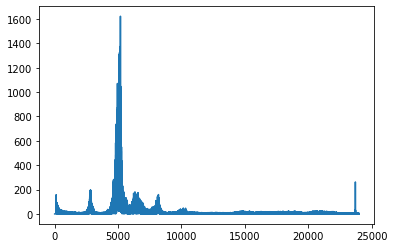
\includegraphics[width=0.75\textwidth]{ex1_crickets_closer_look_1}
        \caption{Смотрим ближе}
        \label{fig:ex1_crickets_closer_look_1}
    \end{figure}
    
    Тут действительно присутствуют много разных частот, однако это не похоже ни на \textquote{розовый} шум, ни на \textquote{белый}. Это так же не походит и на Броуновский шум. Однако, этот \textquote{колокол} кое-на-что похож. Проведем эксперимент.
    
\begin{lstlisting}[language=Python,caption=Проверяем предположение]
import thinkstats2
thinkstats2.NormalProbabilityPlot(spectrum.real)
pyplot.figure()
thinkstats2.NormalProbabilityPlot(spectrum.imag)
\end{lstlisting}
    
    \begin{figure}[H]
        \centering
        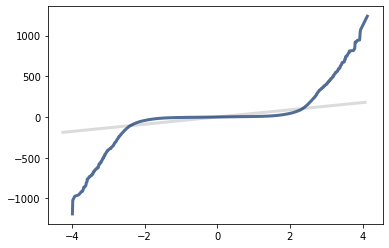
\includegraphics[width=0.75\textwidth]{ex1_crickets_closer_look_2}
        \caption{Вещественная часть}
        \label{fig:ex1_crickets_closer_look_2}
    \end{figure}
    
    \begin{figure}[H]
        \centering
        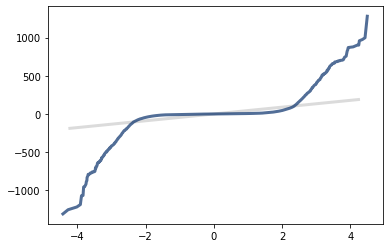
\includegraphics[width=0.75\textwidth]{ex1_crickets_closer_look_3}
        \caption{Мнимая часть}
        \label{fig:ex1_crickets_closer_look_3}
    \end{figure}
    
    Тут как будто бы есть 3 линейных сегмента. Возможно, тут мы имеем дело не с одним нормальным распределением, а несколькими, наложенными друг на дружку.
    
    \begin{figure}[H]
        \centering
        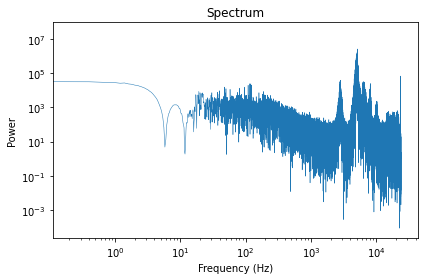
\includegraphics[width=0.75\textwidth]{ex1_crickets_spectrum.png}
        \caption{Спектр сверчков (логарифмический масштаб)}
        \label{fig:ex1_crickets_spectrum}
    \end{figure}
    
    \begin{figure}[H]
        \centering
        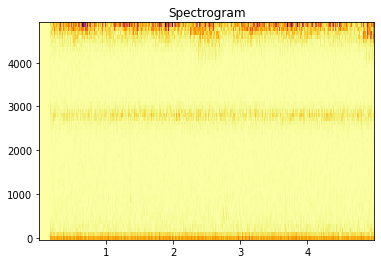
\includegraphics[width=0.75\textwidth]{ex1_crickets_spectrogram.png}
        \caption{Спектрограмма сверчков}
        \label{fig:ex1_crickets_spectrogram}
    \end{figure}
    
    Динамика этого сигнала уже позволяет его назвать шумом, просто он имеет \textquote{предпочтительную} частоты.
    
    \begin{figure}[H]
        \centering
        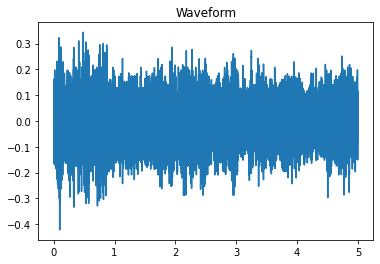
\includegraphics[width=0.75\textwidth]{ex1_crowd_wave.png}
        \caption{Толпа}
        \label{fig:ex1_crowd_wave}
    \end{figure}
    
    \begin{figure}[H]
        \centering
        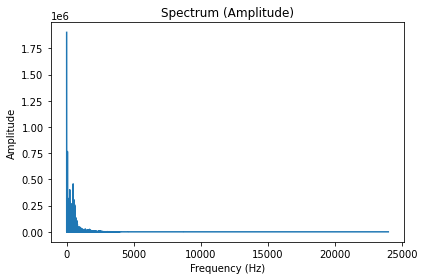
\includegraphics[width=0.75\textwidth]{ex1_crowd_spectrum_amplitude.png}
        \caption{Спектр толпы (линейный масштаб)}
        \label{fig:ex1_crowd_spectrum_amplitude}
    \end{figure}
    
    Вот это уже походит на \textquote{розовый} шум!
    
    \begin{figure}[H]
        \centering
        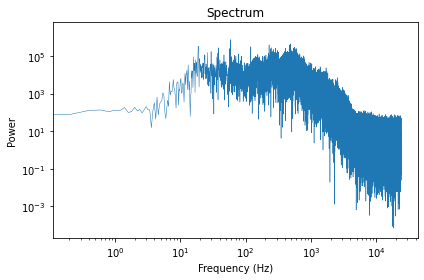
\includegraphics[width=0.75\textwidth]{ex1_crowd_spectrum.png}
        \caption{Спектр толпы (логарифмический масштаб)}
        \label{fig:ex1_crowd_spectrum}
    \end{figure}
    
    Однако данная спектрограмма в логарифмическом масштабе все же дает понять, что перед нами не он.
    
    \begin{figure}[H]
        \centering
        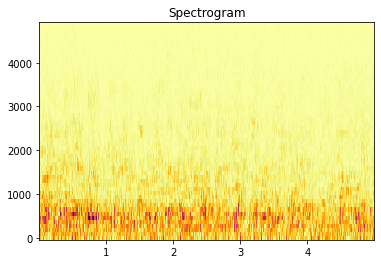
\includegraphics[width=0.75\textwidth]{ex1_crowd_spectrogram.png}
        \caption{Спектрограмма толпы}
        \label{fig:ex1_crowd_spectrogram}
    \end{figure}
    
    Поведение сигнала во времени не оставляет сомнений в том, что 
    
    \chapter{Метод Барлетта}

    Разобъем наш сигнал на отдельные участки, в пределах которых будем брать спектры. 

\begin{lstlisting}[language=Python,caption=Барлетт]
import numpy

wave = read_wave('Sounds/136977__audionautics__crowd-long.wav')

TIME_INTERVAL = 6 * 60
DURATION = 0.01
SAMPLES_COUNT = int(TIME_INTERVAL / DURATION)

summed = numpy.zeros((int(24001 * DURATION + 1)))

for it in range(SAMPLES_COUNT):
    spectrum = wave.segment(start=it * DURATION, duration=DURATION).make_spectrum()
    summed += spectrum.power
    
result = numpy.sqrt(summed / SAMPLES_COUNT)

pyplot.figure()
pyplot.plot(spectrum.fs, result)
pyplot.show()

average_spectrum = Spectrum(result, spectrum.fs, wave.framerate)

loglog = dict(xscale='log', yscale='log')

pyplot.figure()
average_spectrum.plot_power()
decorate(xlabel='Frequency (Hz)', 
         ylabel='Power', 
         **loglog)
\end{lstlisting}
    
    В коде выше можно видеть, как длина временного участка накладывает ограничение на диапазон частот в соответствии с тем, как мы это обсуждали в предыдущей лекции.
    
    Код выше почти эквивалентен коду, предложенному в \sloppy{\texttt{chap04soln.ipynb}} с \sloppy{\texttt{seg\_length}} 512, но работающий чуть побыстрее.
    
    \begin{figure}[H]
        \centering
        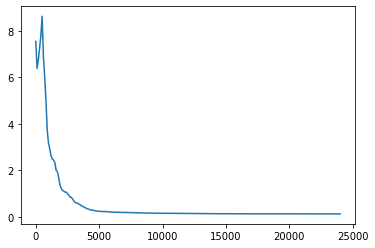
\includegraphics[width=0.75\textwidth]{ex2_average_powers_linear}
        \caption{Линейный масштаб}
        \label{fig:ex2_average_powers_linear}
    \end{figure}
    
    \begin{figure}[H]
        \centering
        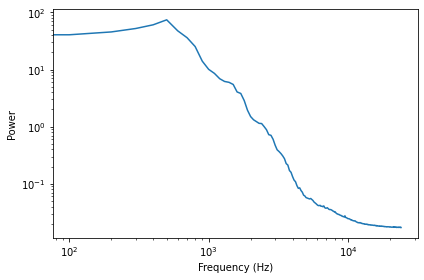
\includegraphics[width=0.75\textwidth]{ex2_average_powers_loglog}
        \caption{Логарифмический масштаб}
        \label{fig:ex2_average_powers_loglog}
    \end{figure}
    
    Видно, что график не похож на горизонтальную прямую или на какую-либо линейную зависимость, при этом сигнал обладает определенной стабильностью во времени (разные частоты неравнозначны, и это сохраняется на протяжении всего времени сигнала).
    
    \chapter{BitCoin}
    
\begin{lstlisting}[language=Python,caption=Загрузка \texttt{DataFrame}]
import pandas
data = pandas.read_csv('Data/BTC_USD_2020-12-31_2021-03-30-CoinDesk.csv')
data
\end{lstlisting}

    \begin{figure}[H]
        \centering
        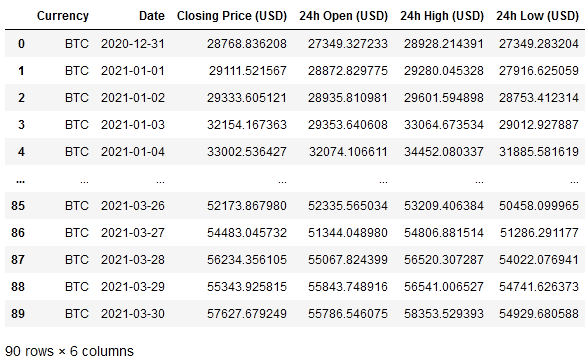
\includegraphics[width=0.75\textwidth]{ex3_data}
        \caption{\texttt{DataFrame}}
        \label{fig:ex3_data}
    \end{figure}
    
    Я скачал данные не за весь период, а только за последний год.
    
\begin{lstlisting}[language=Python,caption=Визуализация]
from thinkdsp import Wave
wave = Wave(data['Closing Price (USD)'], data.index, framerate=1)
wave.plot()
\end{lstlisting}

    \begin{figure}[H]
        \centering
        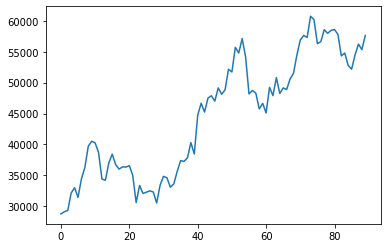
\includegraphics[width=0.75\textwidth]{ex3_wave}
        \caption{Визуализация}
        \label{fig:ex3_wave}
    \end{figure}
    
    Выше мы превратили данные в сигнал, означающий зависимость цены от номера дня.
    
\begin{lstlisting}[language=Python,caption=Спектр]
spectrum = wave.make_spectrum()
spectrum.plot_power()
decorate(xlabel='Frequency (1/days)', **loglog)
\end{lstlisting}

    \begin{figure}[H]
        \centering
        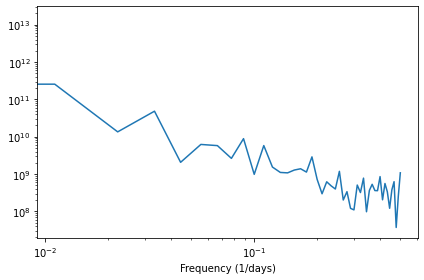
\includegraphics[width=0.75\textwidth]{ex3_spectrum}
        \caption{Спектр}
        \label{fig:ex3_spectrum}
    \end{figure}
    
    Полученный спектр походит на прямую линию, что намекает на возможный \textquote{красный} или \textquote{розовый} шум. Для более точной оценки можно оценить наклон прямой более формально:
    
\begin{lstlisting}[language=Python,caption=Спектр]
spectrum.estimate_slope()[0]
\end{lstlisting}

    Для \textquote{красного} шума характерен наклон -2, поэтому предположу, что это все-таки \textquote{розовый}. Физический же смысл данного спектра в том, что частота изменения стоимости обратно пропорциональна изначимости этих изменений. Другими словами, серьезные изменения остаются достаточно редкими в сравнении с ежедневными флуктуациями.
    
    \chapter{Счетчик Гейгера}
    
    Нам необходимо реализовать сигнал в соответствии с распределением Пуассона, которое имеет следующий вид:
    
    \[
        \begin{aligned}
            P(x) = \frac{\lambda^x e^{-\lambda}}{x!}
        \end{aligned}
    \]
    
    Парамет $\lambda$ соответствует мат. ожиданию и вариации случайной величины ($\lambda = E\xi = E(\xi - E\xi)$). В нашем случае логично говорить об ожидаемом числе попавшихся частиц в неком промежутке времени. Или даже лучше сказать, о среднем количестве встреченных частиц на одно изменение (и измерений в секунду у нас \texttt{framerate} штук).
    
\begin{lstlisting}[language=Python,caption=Реализация]
from thinkdsp import Noise

class MyUncorrelatedPoissonNoise(Noise):
    def evaluate(self, ts):
        ys = numpy.random.poisson(self.amp, len(ts))
        return ys
    
signal = MyUncorrelatedPoissonNoise(amp=0.001)
wave = signal.make_wave(duration=10, framerate=10_000)
wave.make_audio()
\end{lstlisting}

    Прослушать это в \LaTeX нельзя, но звучит правдоподобно.
    
    Можно посмотреть, сколько на самом деле нам прилетело частиц:
    
\begin{lstlisting}[language=Python,caption=Подсчитываем частицы]
sum(wave.ys), 0.001 * 10_000 * 10
\end{lstlisting}

    Получаем на выходе \texttt{(108, 100.0)}, что означает, что примерно столько и прилетело частиц, сколько мы хотели.
    
    Можно еще посчитать пики на вейвформе.
    
\begin{lstlisting}[language=Python,caption=Wave]
wave.plot()
\end{lstlisting}

    \begin{figure}[H]
        \centering
        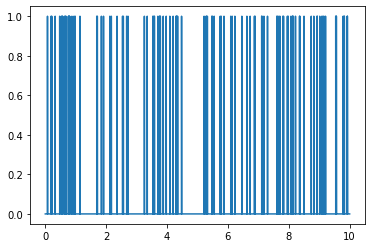
\includegraphics[width=0.75\textwidth]{ex4_wave}
        \caption{Wave}
        \label{fig:ex4_wave}
    \end{figure}
    
    А вот и спектр:
    
\begin{lstlisting}[language=Python,caption=Спектр]
spectrum = wave.make_spectrum()
spectrum.plot_power()
decorate(xlabel='Frequency (Hz)',
         ylabel='Power',
         **loglog)
\end{lstlisting}

    \begin{figure}[H]
        \centering
        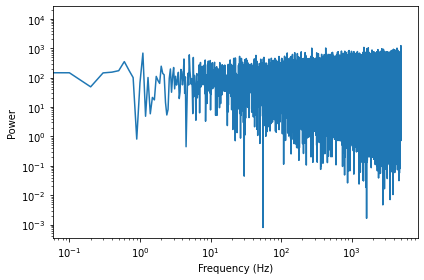
\includegraphics[width=0.75\textwidth]{ex4_spectrum}
        \caption{Спектр}
        \label{fig:ex4_spectrum}
    \end{figure}
    
    Он походит на прямую горизонтальную линию, а оценка его наклона показывает величину, близкую к 0. Похоже, что это \textquote{белый} шум.
    
    \chapter{Алгоритм Восса-МакКартни}
    
    Это просто более хороший алгоритм для генерации \textquote{розового} шума.
    
\begin{lstlisting}[language=Python,caption=Алгоритм]
def voss(rows, columns=16):
    array = numpy.empty((rows, columns))
    array.fill(numpy.nan)
    
    array[0, :] = numpy.random.random(columns)
    array[:, 0] = numpy.random.random(rows)
    
    target_columns = numpy.random.geometric(0.5, rows)
    target_columns[target_columns >= columns] = 0
    
    target_rows = numpy.random.randint(rows, size=rows)
    
    array[target_rows, target_columns] = numpy.random.random(rows)

    dataframe = pandas.DataFrame(array)
    dataframe.fillna(method='ffill', axis=0, inplace=True)
    
    total = dataframe.sum(axis=1)
    return total.values

wave = Wave(voss(11025))
wave.unbias()
wave.plot()
wave.make_audio()
\end{lstlisting}

    Идея алгоритма заключается в сложении нескольких последовательностей случайных чисел, изменяющихся с разной частотой (эти числовые последоваьельности представлены столбцами, вдоль которых потом производится суммирование).

    \begin{figure}[H]
        \centering
        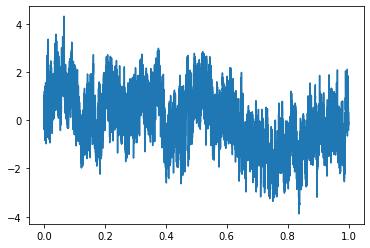
\includegraphics[width=0.75\textwidth]{ex5_wave}
        \caption{Сигнал}
        \label{fig:ex5_wave}
    \end{figure}
    
\begin{lstlisting}[language=Python,caption=Спектр]
spectrum = wave.make_spectrum()
spectrum.hs[0] = 0
spectrum.plot_power()
decorate(xlabel='Frequency (Hz)',
         **loglog)
\end{lstlisting}

    \begin{figure}[H]
        \centering
        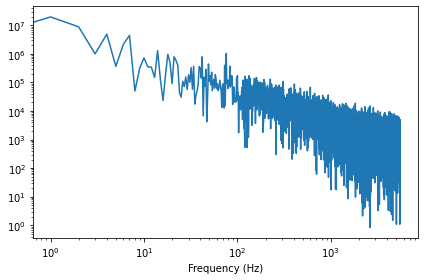
\includegraphics[width=0.75\textwidth]{ex5_spectrum}
        \caption{Спектр}
        \label{fig:ex5_spectrum}
    \end{figure}
    
    Виднеется прямая. Оценка ее наклона дает величину, близкую к -1, что говорит о том, что перед нами точно \textquote{розовый} шум.
    
    \printbibliography
    
\end{document}
